


\documentclass[conference]{IEEEtran}
\usepackage{blindtext, graphicx}

% *** MISC UTILITY PACKAGES ***
%
%\usepackage{ifpdf}
% Heiko Oberdiek's ifpdf.sty is very useful if you need conditional
% compilation based on whether the output is pdf or dvi.
% usage:
% \ifpdf
%   % pdf code
% \else
%   % dvi code
% \fi
% The latest version of ifpdf.sty can be obtained from:
% http://www.ctan.org/tex-archive/macros/latex/contrib/oberdiek/
% Also, note that IEEEtran.cls V1.7 and later provides a builtin
% \ifCLASSINFOpdf conditional that works the same way.
% When switching from latex to pdflatex and vice-versa, the compiler may
% have to be run twice to clear warning/error messages.

% *** GRAPHICS RELATED PACKAGES ***
%
\ifCLASSINFOpdf
  % \usepackage[pdftex]{graphicx}
  % declare the path(s) where your graphic files are
  % \graphicspath{{../pdf/}{../jpeg/}}
  % and their extensions so you won't have to specify these with
  % every instance of \includegraphics
  % \DeclareGraphicsExtensions{.pdf,.jpeg,.png}
\else
  % or other class option (dvipsone, dvipdf, if not using dvips). graphicx
  % will default to the driver specified in the system graphics.cfg if no
  % driver is specified.
  % \usepackage[dvips]{graphicx}
  % declare the path(s) where your graphic files are
  % \graphicspath{{../eps/}}
  % and their extensions so you won't have to specify these with
  % every instance of \includegraphics
  % \DeclareGraphicsExtensions{.eps}
\fi
% graphicx was written by David Carlisle and Sebastian Rahtz. It is
% required if you want graphics, photos, etc. graphicx.sty is already
% installed on most LaTeX systems. The latest version and documentation can
% be obtained at: 
% http://www.ctan.org/tex-archive/macros/latex/required/graphics/
% Another good source of documentation is "Using Imported Graphics in
% LaTeX2e" by Keith Reckdahl which can be found as epslatex.ps or
% epslatex.pdf at: http://www.ctan.org/tex-archive/info/
%
% latex, and pdflatex in dvi mode, support graphics in encapsulated
% postscript (.eps) format. pdflatex in pdf mode supports graphics
% in .pdf, .jpeg, .png and .mps (metapost) formats. Users should ensure
% that all non-photo figures use a vector format (.eps, .pdf, .mps) and
% not a bitmapped formats (.jpeg, .png). IEEE frowns on bitmapped formats
% which can result in "jaggedy"/blurry rendering of lines and letters as
% well as large increases in file sizes.
%
% You can find documentation about the pdfTeX application at:
% http://www.tug.org/applications/pdftex


% *** MATH PACKAGES ***

\usepackage[cmex10]{amsmath}

% *** SPECIALIZED LIST PACKAGES ***
%
%\usepackage{algorithmic}
% algorithmic.sty was written by Peter Williams and Rogerio Brito.
% This package provides an algorithmic environment fo describing algorithms.
% You can use the algorithmic environment in-text or within a figure
% environment to provide for a floating algorithm. Do NOT use the algorithm
% floating environment provided by algorithm.sty (by the same authors) or
% algorithm2e.sty (by Christophe Fiorio) as IEEE does not use dedicated
% algorithm float types and packages that provide these will not provide
% correct IEEE style captions. The latest version and documentation of
% algorithmic.sty can be obtained at:
% http://www.ctan.org/tex-archive/macros/latex/contrib/algorithms/
% There is also a support site at:
% http://algorithms.berlios.de/index.html
% Also of interest may be the (relatively newer and more customizable)
% algorithmicx.sty package by Szasz Janos:
% http://www.ctan.org/tex-archive/macros/latex/contrib/algorithmicx/

% *** ALIGNMENT PACKAGES ***
%
\usepackage{array}
% Frank Mittelbach's and David Carlisle's array.sty patches and improves
% the standard LaTeX2e array and tabular environments to provide better
% appearance and additional user controls. As the default LaTeX2e table
% generation code is lacking to the point of almost being broken with
% respect to the quality of the end results, all users are strongly
% advised to use an enhanced (at the very least that provided by array.sty)
% set of table tools. array.sty is already installed on most systems. The
% latest version and documentation can be obtained at:
% http://www.ctan.org/tex-archive/macros/latex/required/tools/


%\usepackage{mdwmath}
%\usepackage{mdwtab}
% Also highly recommended is Mark Wooding's extremely powerful MDW tools,
% especially mdwmath.sty and mdwtab.sty which are used to format equations
% and tables, respectively. The MDWtools set is already installed on most
% LaTeX systems. The lastest version and documentation is available at:
% http://www.ctan.org/tex-archive/macros/latex/contrib/mdwtools/


% IEEEtran contains the IEEEeqnarray family of commands that can be used to
% generate multiline equations as well as matrices, tables, etc., of high
% quality.


%\usepackage{eqparbox}
% Also of notable interest is Scott Pakin's eqparbox package for creating
% (automatically sized) equal width boxes - aka "natural width parboxes".
% Available at:
% http://www.ctan.org/tex-archive/macros/latex/contrib/eqparbox/





% *** SUBFIGURE PACKAGES ***
\usepackage[tight,footnotesize]{subfigure}
% subfigure.sty was written by Steven Douglas Cochran. This package makes it
% easy to put subfigures in your figures. e.g., "Figure 1a and 1b". For IEEE
% work, it is a good idea to load it with the tight package option to reduce
% the amount of white space around the subfigures. subfigure.sty is already
% installed on most LaTeX systems. The latest version and documentation can
% be obtained at:
% http://www.ctan.org/tex-archive/obsolete/macros/latex/contrib/subfigure/
% subfigure.sty has been superceeded by subfig.sty.



%\usepackage[caption=false]{caption}
%\usepackage[font=footnotesize]{subfig}
% subfig.sty, also written by Steven Douglas Cochran, is the modern
% replacement for subfigure.sty. However, subfig.sty requires and
% automatically loads Axel Sommerfeldt's caption.sty which will override
% IEEEtran.cls handling of captions and this will result in nonIEEE style
% figure/table captions. To prevent this problem, be sure and preload
% caption.sty with its "caption=false" package option. This is will preserve
% IEEEtran.cls handing of captions. Version 1.3 (2005/06/28) and later 
% (recommended due to many improvements over 1.2) of subfig.sty supports
% the caption=false option directly:
%\usepackage[caption=false,font=footnotesize]{subfig}
%
% The latest version and documentation can be obtained at:
% http://www.ctan.org/tex-archive/macros/latex/contrib/subfig/
% The latest version and documentation of caption.sty can be obtained at:
% http://www.ctan.org/tex-archive/macros/latex/contrib/caption/




% *** FLOAT PACKAGES ***
%
%\usepackage{fixltx2e}
% fixltx2e, the successor to the earlier fix2col.sty, was written by
% Frank Mittelbach and David Carlisle. This package corrects a few problems
% in the LaTeX2e kernel, the most notable of which is that in current
% LaTeX2e releases, the ordering of single and double column floats is not
% guaranteed to be preserved. Thus, an unpatched LaTeX2e can allow a
% single column figure to be placed prior to an earlier double column
% figure. The latest version and documentation can be found at:
% http://www.ctan.org/tex-archive/macros/latex/base/



%\usepackage{stfloats}
% stfloats.sty was written by Sigitas Tolusis. This package gives LaTeX2e
% the ability to do double column floats at the bottom of the page as well
% as the top. (e.g., "\begin{figure*}[!b]" is not normally possible in
% LaTeX2e). It also provides a command:
%\fnbelowfloat
% to enable the placement of footnotes below bottom floats (the standard
% LaTeX2e kernel puts them above bottom floats). This is an invasive package
% which rewrites many portions of the LaTeX2e float routines. It may not work
% with other packages that modify the LaTeX2e float routines. The latest
% version and documentation can be obtained at:
% http://www.ctan.org/tex-archive/macros/latex/contrib/sttools/
% Documentation is contained in the stfloats.sty comments as well as in the
% presfull.pdf file. Do not use the stfloats baselinefloat ability as IEEE
% does not allow \baselineskip to stretch. Authors submitting work to the
% IEEE should note that IEEE rarely uses double column equations and
% that authors should try to avoid such use. Do not be tempted to use the
% cuted.sty or midfloat.sty packages (also by Sigitas Tolusis) as IEEE does
% not format its papers in such ways.





% *** PDF, URL AND HYPERLINK PACKAGES ***
%
\usepackage{url}
% url.sty was written by Donald Arseneau. It provides better support for
% handling and breaking URLs. url.sty is already installed on most LaTeX
% systems. The latest version can be obtained at:
% http://www.ctan.org/tex-archive/macros/latex/contrib/misc/
% Read the url.sty source comments for usage information. Basically,
% \url{my_url_here}.





% *** Do not adjust lengths that control margins, column widths, etc. ***
% *** Do not use packages that alter fonts (such as pslatex).         ***
% There should be no need to do such things with IEEEtran.cls V1.6 and later.
% (Unless specifically asked to do so by the journal or conference you plan
% to submit to, of course. )


% correct bad hyphenation here
\hyphenation{op-tical net-works semi-conduc-tor}


\begin{document}
%
% paper title
% can use linebreaks \\ within to get better formatting as desired
\title{A Comfortable Overlay for Economy Airline Seating}


% author names and affiliations
% use a multiple column layout for up to three different
% affiliations
\author{\IEEEauthorblockN{Luke Wiwatowski}
\IEEEauthorblockA{Faculty of Science, Engineering and Technology\\
Swinburne University of Technology\\
Melbourne Australia\\
1745867@student.swin.edu.au}
\and
\IEEEauthorblockN{Wanicha Timsuren}
\IEEEauthorblockA{Faculty of Science, Engineering and Technology\\
Swinburne University of Technology\\
Melbourne Australia\\
6652972@student.swin.edu.au}
}


\maketitle

\begin{abstract}
Economy airline seating has a widespread reputation for being cramped and uncomfortable. This research project was an effort to explore whether the comfort conditions could be improved. Solidworks was used to model the cushion and seating load to iteratively design a cushion that could be used to create a more comfortable sitting experience on commercial economy airline seats. It was found that an ideal cushion design had a lower Young's modulus and a contoured shaped to fit the buttocks. The simulations performed to date showed that the investigated cushion designs had not met a target peak stress below 12kPa, which has previously found to be a threshold for higher comfort levels. Further research is required to investigate improved designs.
\end{abstract}

\begin{IEEEkeywords}
Airline Seating, comfort, cushion, stress distribution, Solidworks.
\end{IEEEkeywords}

\tableofcontents

\section{Introduction}

How can an adjustable smart device overlay for airline seating be modelled to help increase the comfort for passengers within the current regulatory and carrier limitations?

Airline economy seating does not have a high reputation in terms of comfort. There is a pervasive view that it is cramped and not focused on the needs of the passengers \cite{SKYTRAXOnline2014}. This is a consistent theme across airlines and manufacturers and, as such, warrants investigation into the causes of this and how it could be improved. This research endeavours to improve comfort for economy seating in current airlines. The method pursued will be to design a commercially available product such as a cushion or overlay which the passengers can use to augment their commercial airline seating experience. Comfort is a multifaceted subject and covers many topics. To frame this subject within an engineering perspective there will be particular focus on measurable engineering phenomena such as stress, force and friction. The factors that can be objectively measured and improved upon hold the most priority when framed from an engineering perspective so these factors will be focused on. On a more economical thread the product design has to stay within a reasonable cost as the design will have to be attractive to passengers as an investment in their comfort. It must also be durable enough to last several flights such as current products on the market for similar purposes.

The reasons for airlines's reputation for uncomfortable and cramped economy seating is varied. There are many criteria that an airline seat must achieve before it can be used for commercial purposes and the implementation of these may play into the lack of detail to comfort. Strict safety standards mandated by airline governing bodies must be adhered to \cite{CornellLaw}. These safety standards include force, motion and flammability criteria. Without these standards adhered to commercial airlines are forbidden to use those seats until they pass these safety tests. There are also no mandated comfort standards in terms of dimensions or any other factors and these are wholly decided by the manufacturers, airlines and their requisite governing bodies \cite{CASA}. In addition the economics and profitability of the manufacturers and airlines are also a major consideration. Since airlines and manufacturers run under the world's largely capitalist system profit is essentially the highest consideration. As such capacity becomes a large driving factor for design and the profitability of these companies. With these factors combined the comfort of the passenger can slip down the list of priorities for airlines and seat manufacturers. Additionally there appears to be largely a race to the bottom for airlines in that economy customers are generally focused on price and only notice the conditions of the airline seating after the tickets are purchased and they are already committed to the flight. So airlines have little incentive to provide a significantly passenger experience to competitors and therefore the quality of economy seating drifts lower and lower.

Measuring comfort can be difficult since it is a very subjective matter with many factors involved. Not only are there psychological factors and individual preferences, additionally humans differ in their body shape and stature. Therefore a lot of subjective factors are prevalent when attempting to measure comfort. To simplify this problem there are some factors that can be objectively measured such as stress, force and dimensioning for a majority of the flying population \cite{HermanMiller2013}. There is research to conclude that fluid flow in the body is a good indicator of overall comfort, if the flow is too restricted there is a strong correlation between chair design and discomfort. The current research indicates that at a stress value greater than 12 kPa fluid flow in the body is restricted and long term comfort diminishes \cite{Nigel2002}. As such this value of 12 kPa has been targeted to provide a good measure as to how the design of the overlay performs. If an overlay or cushion can reduce the peak stresss to below this value then the design can be considered successful. Therefore essentially the design is an exercise in stress and force redistribution, which matches well with framing the research in engineering terms.

This research will see benefits in a few areas, economically, physically and mentally. The benefits extend not just to the individual but perhaps also to the airlines and manufacturers themselves. From an individual perspective this allows for a more comfortable flight experience with a minimal cost outlay, without having to pay the relatively large costs for seating upgrades. The product can help stave off the risks of long term inactivity such as deep vein thrombosis. On another level this product may help encourage those who would otherwise not fly long distances to do so. The flow on affects of this are varied, such as more customers and, therefore, more revenue for airlines. As well as social reasons such as family and friends who otherwise would not meet each other physically given that opportunity. Of course the benefit for airlines and manufacturers is that this research assists them in creating perhaps a better comfort experience. If there are valid and easy to implement recommendations in this research then the manufacturers and airlines have been saved doing the research and development themselves.

\section{Literature Review}
Current research on this subject can be structured into four broad categories. These explore the current constraints and regulations on airline seating, the human factors of airline seating and sitting position more generally, current available products and designs which may aim to address a similar goal to this research as well as the materials and their properties needed to achieve the end goal. The literature is comprehensive in some parts but also slightly lacking in others, related topics were needed to get a better idea of how comfort is measured and how to implement this information.
    
    \subsection{Rules and Regulations}
    Airline seats have rules and regulations which must be adhered to, however these regulations mostly involve the safety specifications \cite{CornellLaw}. There are no regulations which specify minimum dimensions for comfort with these being agreed upon internally between the relevant airline manufacturer and its requisite governing body \cite{CASA}.In this particular research the focus will be on Boeing and the Federal Aviation Authority (FAA). Manufacturers must submit their designs for safety testing to the FAA for certification \cite{TSO}. These tests cover safety standards for maximum forces, stresss and fire resistance \cite{Housel2004}. This can take a long time and as such it appears the manufacturers, whether on purpose or not, push the priority of comfort behind the priorities of safety testing and carriers' capacity needs. Additionally the economics and efficiencies of flying see a large focus on reducing the weight of the seats, any small decrease per seat can see large gains economically \cite{RECARO2010}.
    
    The product itself will have to work within the dimensions of current airline seating standards (see table \ref{dimensions}) which can vary from carrier to carrier. Information for these dimensions can be quite hard to confirm so the product will also have to be flexible enough to fit within these parameters.
        
\begin{table}[!t]
    \centering
    \caption{Typical airline seating dimensions
    \cite{Goonetilleke2001,SKYTRAXOnline2014}}
    \label{dimensions}
    \begin{tabular}{l p{3cm} c}
    \hline
    Dimension      & Description                                                        & Typical Distance \\ \hline \hline
    Pitch          & Distance between the same point from one seat to the seat in front & 76-81 cm         \\ \hline
    Width          & Distance from armrest to armrest                                   & 43-46 cm         \\ \hline
    Depth          & Distance from front of seat to back                                & 42-50 cm         \\ \hline
    Angle/Rake     & Angle of the seat relative to horizontal                           & Up to 15 degrees \\ \hline
    Armrest height & Distance from top of cushion to top of armrest                     & Data Unavailable \\ \hline
    Back height    & Height of the back rest from the top of the seat height            & Data Unavailable \\ 
    \end{tabular}
\end{table}



\begin{figure}[!t]
\centering
    \caption{Typical economy seat dimensions}
 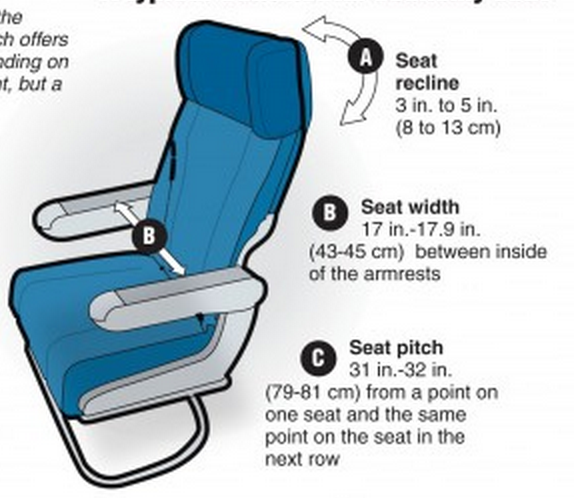
\includegraphics[width=2.5in]{pics/seatSpecs.png} 
    \label{seatSpecs}
\end{figure}

    \subsection{Ergonomics and Human Factors}
    The ergonomics of sitting for long periods has been studied for various purposes and there appears to be some consensus on what constitutes a relatively comfortable chair. Generally speaking a comfortable chair spreads the load of the body over as large a surface area as possible with high stress points preferably focused on the bony protrusion on the bottom of the pelvic bone known as the ischial tuberosities \cite{HermanMiller2013}. Overall stress on at any point should not exceed 12 kPa as this is the stress that cuts off fluid flow and circulation in the body \cite{Nigel2002}.This gives a good target to aim for as it is more absolute than data from questionnaires and surveys.
    
    Other important considerations are the addition of well positioned footrests, backrests and armrests \cite{Graf1993, drury1982} which allow for further weight redistribution and body adjustment. They have been shown to increase comfort considerably given the placement of them is optimised for the sitter. The limitations with these is that it becomes difficult to place these various rests in a positions which satisfies the 95th percentile \cite{drury1982}.
    
    This also leads into the theory of dynamic sitting which suggests that for long periods of time a single sitting position cannot be ideal and the sitter must change position to allow for good circulation and redistribute muscle strain \cite{Stockton2008}. These changes should generally occur every fifteen minutes or so however able bodied human beings will generally do this unconsciously due to the encouragement of the body producing aches and pains. For the wheelchair bound it has been shown that dynamic cushions, which change shape themselves to encourage dynamic seating, can be beneficial to encourage fluid flow within the body \cite{Stockton2008}.
        
    \subsection{Current Designs}
    There are currently some products that claim to assist with comfort on long haul flights as well as a few scattered patents \cite{duncan2003inflatable, treacy1967inflatable}. The bulk of these appear to be low quality and have varying claims in their effectiveness. Patents by their nature do not claim huge benefits but rather just outline ideas and the current designs available do not appear to be backed by evidence for their claims. So it seems there may be a niche to create a product that is more evidence based.
    
    There are some studies on related topics which have may have applicable ideas to the current task. There are some papers involving car seats \cite{Verver2005, Grujicic2009} which offer good evidence into comfort. They also provide valuable information on computer modelling of seats and how to measure human interactions with them. Another related topic which has proven to be useful has been the industry of wheelchairs and the infirm. Care must be taken with this data since experiments have shown to have differing results depending on whether the test subjects were in fact disabled or not \cite{Hobson1992}. Keeping this in mind however the products take greater care to provide comfort and less damage to the body. The theory of dynamic seating is perhaps a useful one, it states, as previously noted, that no static position will remain comfortable, instead the person sitting will naturally (assuming they are able bodied) move and shift position due to encouragement from natural aches and pains \cite{Graf1993}. This helps the body circulate better and prevents problems seen in the disabled such as bed sores \cite{Stockton2008}. Using this theory there are various dynamic cushions (see figure \ref{cushion}) on the market designed for use for people with disabilities \cite{BartramAssociatesLtd2015}. They generally consist of a cushion consisting of separated air pockets which slowly inflate and deflate allowing for better circulation within the body and allowing for stress differentials to propagate about the body rather than stay in one area. They tend to retail in the high hundreds of dollars to the low thousands. This may be a useful avenue to pursue, if costs can be compressed enough perhaps a commercial version for the general public may be viable.
    
\begin{figure}[!t]
\centering
    \caption{A dynamic cushion \cite{BartramAssociatesLtd2015}}
 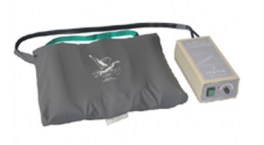
\includegraphics[width=2.5in]{pics/dynamicCushion.png} 
    \label{cushion}
\end{figure}

    \subsection{Materials}
    The materials used for our design are the options of three broad categories. Each with specific advantages and disadvantages. Table \ref{proscons} shows a summary of each material.
        
\begin{table}[!t]
\centering
    \caption{Advantages and disadvantages of certain material types}
    \label{proscons}
\begin{tabular}{cll}
\hline
Material & \multicolumn{1}{c}{Advantages}                                                                       & \multicolumn{1}{c}{Disadvantages}                                                                     \\ \hline \hline
Foam     & \begin{tabular}[c]{@{}l@{}}Light\\ Cheap\\ Good heat transfer properties\end{tabular}                 & \begin{tabular}[c]{@{}l@{}}Limitations in compression\\ Quality and durability variable\end{tabular}  \\ \hline
Gel      & \begin{tabular}[c]{@{}l@{}}Comfortable\\ Malleable\\ Recommended by health proffesionals\end{tabular} & \begin{tabular}[c]{@{}l@{}}Leakages can occur\\ Heavier\\ Viscosity can be disconcerting\end{tabular} \\ \hline
Air      & \begin{tabular}[c]{@{}l@{}}Light\\ Constant density\\ Cell design\end{tabular}                        & \begin{tabular}[c]{@{}l@{}}Costs are high\\ Can be unstable to sit on\\ Can be punctured    \end{tabular} 
\end{tabular} 
\end{table}

        \subsubsection{Polyurethane Foam}
        Polyurethane foam has the strongest advantages of the options. The properties which make it desirable are it's cost, weight and compressibility. It generally follows the stress strain rule (see equation \ref{stressstrain}). There also some disadvantages however.
        
        \begin{equation}
        \label{stressstrain}
        \sigma_{x} = E\varepsilon_{x}
        \end{equation}

The density is important for polyurethane foam specification. It is an important indicator of foam performance with regard to comfort, support and durability. It is also an indicator of the relative economics of the foam \cite{PolyurethaneFoamAssociation1991}. High-density foams can be produced to be very soft. Low-density foams can be very firm. High-density foam products generally offer great deal of support, but they may actually be fairly soft foams (Volume I, Number 2, May 1991). Studies have shown that the most comfortable seating with a foam cushion is a medium density polyurethane with compression no greater than two to three centimetres \cite{drury1982}. Foam, in contrast to the other options, is compressible and suffers from reaching a point of incompressibility. If this point is reached seating will feel much more uncomfortable \cite{Nigel2002} as the foam has no where to disperse sideways. There are possible ways to get around this limitation, such as slicing the foam into upright square prisms. This however can affect durability.

Another important property of foam as compared to other options is that foam does not have a strictly linear compressibility pattern. Initially foam has a linear compression curve but then there is a point of incompressibility where the properties change sharply. Ideally this point of incompressibility should not be reached to achieve maximum comfort values.
%need to insert references for incompressibility here.

\begin{table}[!t]
    \centering
    \caption{Typical properties of polyurethane foam \cite{Patel2008}}
    \label{properties}
    \begin{tabular}{c c}
    \hline
    Mechanical Properties         	& Metric 				\\ \hline \hline
    Young's Modulus                   	& 8 kN/m\textsuperscript{2}  - 150 MN/m\textsuperscript{2}	 \\ \hline
    Poisson's Ratio                    	& 0.300 - 0.750         		\\ 
    \end{tabular}
\end{table}

        \subsubsection{Gel}
        Gel seat cushion are generally recommended by Health professionals and are used extensively by wheelchair users \cite{Stockton2008}. The development of the gel seat cushion is fuelled by the need for a comfortable and healthy seating option for car, office and the infirm. They ensure maximum comfort for a long period of time. The extra-wide design fits any body type and offers full protection from direct stress. The ideal is for long road trips, flights, picnics, ball games, and camping. They are ideally placed against the backrest. Support comes from the lumbar or lower back region, effectively eliminating lower back pain (Brooks K, 2013). The general design is of separate pockets with highly viscous gel in each with the skin made of a tough rubber. This is generally regarded as giving the best comfort however there are some disadvantages. These are the heaviest of all cushions and can be prone to leaking \cite{Arthanat2006}. Hence their use in applications which do not require lots of travelling. As such this material may not be suitable for the needs of the project.
        
        \subsubsection{Air}
        Air-inflated seat cushion consist of cells allowing air to flow between each of them and inflation holes. Inner parts of the cushion are connected. There are air outlets and passages for air to flow between cells. When a driver moves onto the cushion, the shape of the cushion will change accordingly. With air flowing between cells, the air-inflated cells act as shock absorbers with damping characteristics depending on cell pressure, cell size and air transfer rate between cells \cite{Xinglei2010}. This design is generally the one which can easily incorporate dynamic seating \cite{BartramAssociatesLtd2015}. Air suffers some of the downsides of gel cushions but does manage to stay light, this however introduces issues with stability, where the cushion can easily shift and collapse under uneven pressure \cite{Arthanat2006}. The advantage of both gel and air cushioning is that when compressed the outer skin allows the fluid inside to disperse horizontally and should theoretically create a more comfortable impression \cite{Nigel2002}. These are however not insurmountable problems for foam to overcome.
        
    \subsection{Other Considerations}
        \subsubsection{Thermal Conductivity}
        The total thermal conductivity is the sum of the conductivities of both the gas and solid phase plus the thermal conductivity due to convection and radiation. The thermal conductivity is very low for polymer foams because the amount of solid in the foam is very small. The thermal conductivity has a minimum at a certain density. At low densities the radiative component is more dominant since the cell size is larger, and so is the convective component. At high densities the number of cell walls and the thickness of them is higher so the radiative component is less important, but the heat transfer through the solid phase becomes more dominant \cite{sivertsen2007polymer}.
        
        \subsubsection{Cushion Covering}
        The selection of an appropriate cushion cover can influence seating – for example a smooth surface cover, compared with a towelling-type or wool-pile cover, may ease sideways transfers for those who are weak or with a degenerative neurological condition. Maintenance or loss of body heat may also influence the selection of cover materials. Where less body heat is generated for example in the frail elderly a wool-pile or towelling cover may be preferable whereas in young active wheelchair users similar covers may promote heat and moisture build-up. For the incontinent individual ease of cleaning the cover is crucial and where the cover can be detached from the cushion a covered zip is required. As with the care of the cushion itself the individual, their family and/or carer require to be informed regarding the care of the cushion cover. This education needs to cover how to detach, launder and reapply the cover taking account of instructions that may be printed on the cover or cushion for example location of the front or top surface of the cushion or cover \cite{TissueViabilitySociety2013}.


\section{Methodology}

Solidworks simulations were used as the preferred method for iterative design of the cushion. The reason for this decision had some varying justifications. Firstly Solidworks is the de facto standard for many engineering projects involving computer aided design, it is also software which the members of this research project were familiar with already. Secondly using computer aided design allowed for quick iteration of material properties and designs, effectively allowing testing of more combinations without having to physically build the models. Finally the results were repeatable and objective without having to rely on subjective methods like surveys and questionnaires. Finite element analysis was used to determine the maximum stress felt by the human lower torso simulation on a variety of cushions shapes with varying material properties. The simulation used a simplified buttocks model with dimensions generally following an average human being. A downward force was applied to the simulated buttocks at the equivalent to an 80kg human being. The analysis done was a static FEA model as there are assumed to be negligible dynamic forces when a person is sitting down. The cushion designs were constrained at the base to not move during the simulation, the buttocks was only allowed to translate downwards and sideways movement was constrained. The material properties and cushion shape were iterated to attempt to design a model that minimised peak stresses on the surface of the buttocks to below 12 kPa.

\begin{figure}[!t]
\centering
 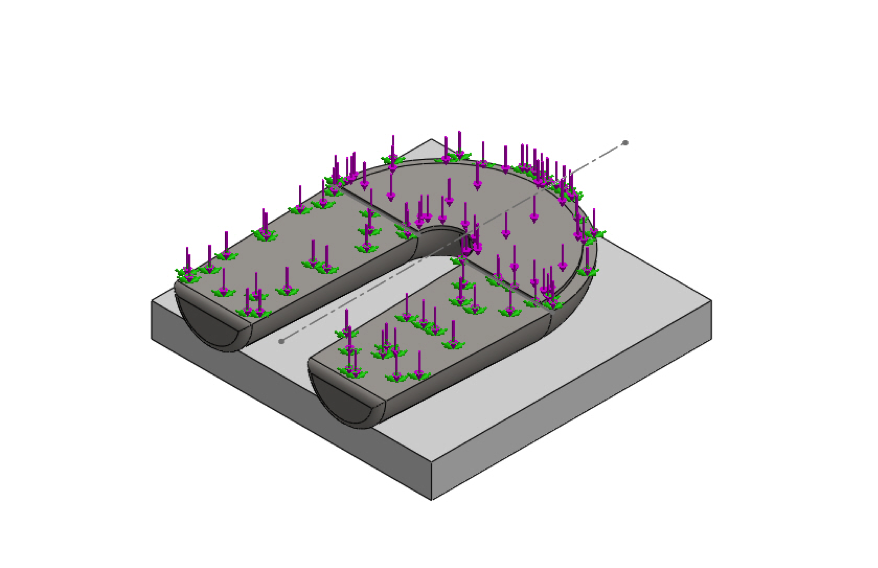
\includegraphics[width=2.5in]{pics/simulation.png}
    \caption{Simulation with forces and restraints}
    \label{simulation}
\end{figure}

The model buttocks was kept as a simple model with few surfaces and the shape was based on pressure profiles of buttocks from similar studies \cite{HermanMiller2013,Grujicic2009}. The simple model allowed for simpler contact points and easier iteration on the cushion design. A uniform force was distributed on the top surface and a surface to surface contact set was used for higher accuracy (see figure \ref{simulation}). Mesh settings were set a medium density so as to quickly iterate on materials and designs without using too much computational power. 


The first designs of the cushion remained a simple rectangular prism which eliminated variables in the contour of the cushion. The cushion was constrained on the bottom surface and the buttocks was constrain to translate vertically only. This way the static analysis could focus on the ideal material properties to achieve the desired target peak stress. There were two critical properties that were varied to achieve different results for the static analysis, the Young's modulus and Poisson's ratio. The Young's modulus is also known as the modulus of elasticity and is a measure in N/m\textsuperscript{2} of the stresses in a material vs the strain. A higher Young's modulus means the material will distort less with stress while a low modulus means more distortion with the same stress. The range of values that polyurethane foam can have for the Young's modulus was quite large, ranging between 8 kN/m\textsuperscript{2} to 150 MN/m\textsuperscript{2} \cite{Patel2008}. The team decided to test Young's modulus at a logarithmic scale between 10 kN/m\textsuperscript{2} and 10 MN/m\textsuperscript{2} giving a good idea of how the material will behave between such large values. Poisson's ratio is a measure of how much a material will expand in one dimension when compressed in another dimension. Solidworks was limited to simulating Poisson's ratio in a range of 0.01 to 0.45. 



After the iterative material property design process was completed on the flat cushion iterative design then proceeded contouring the cushion to better fit the simulated buttocks. The contours on the cushion were based on results from previous studies and trial and error design. The contoured cushions were tested using the optimal material properties determined in the first part of the methodology. The best of these designs can be seen in figure
%insert figure and cross reference back to above paragraph.


\section{Results}

The full results can be viewed in appendix X however the following will show the most indicative results. The testing showed the compression and stress results on the surface of the simulated buttocks. These surface stresses were collated and graphed to show the main effects of varying the material properties. As stated previously the Young's modulus and Poisson's ratio were the properties varied to achieve the listed results. In figures \ref{stress} and \ref{maxstress} results from opposing ends of the scale of stress distribution can be seen. Although in some results the stress distribution over the top section of the buttocks model experienced very high stress levels those were generally ignored in favour of the stress values of over the underside of the model most affected by the cushion.

Figure \ref{maxstress} shows the simulation with the highest peak stress values on the underside of the buttocks model. As pointed out previously the highest stress values can be seen in the area where the ischial tuberosities would be located. The peak stresses here were at 169 kN/m\textsuperscript{2}. This was a good indication that the simulation was a valid one which mimics the real world. The material properties configuration for this test was a Poisson's ratio of 0.49 and a Young's modulus of 10 MN/m\textsuperscript{2}.

Figure \ref{stress} shows the simulation with the lowest peak stress values on the underside of the buttocks model. In this simulation the peak stress did not exceed 22 kN/m\textsuperscript{2}. The material properties configuration for this simulation was a Poisson's ratio at 0.25 and a Young's modulus at 10 kN/m\textsuperscript{2}.

\begin{figure}[!t]
\centering
 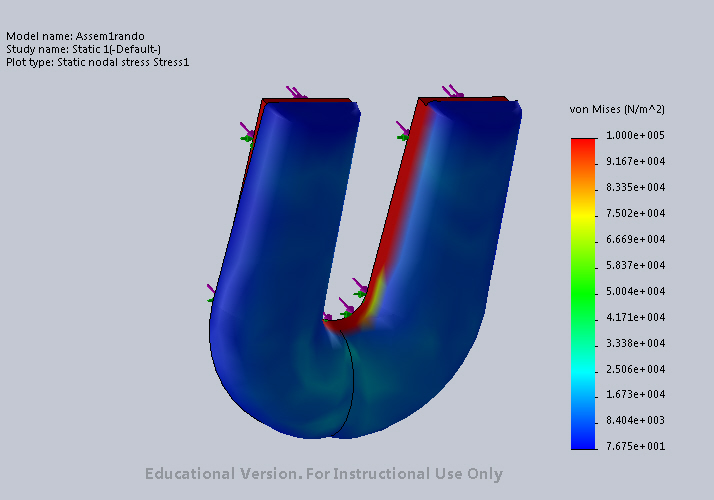
\includegraphics[width=2.5in]{pics/ButtocksPressure.jpg}
    \caption{stress results for simulation with minimum peak stress}
    \label{stress}
\end{figure}

\begin{figure}[!t]
\centering
 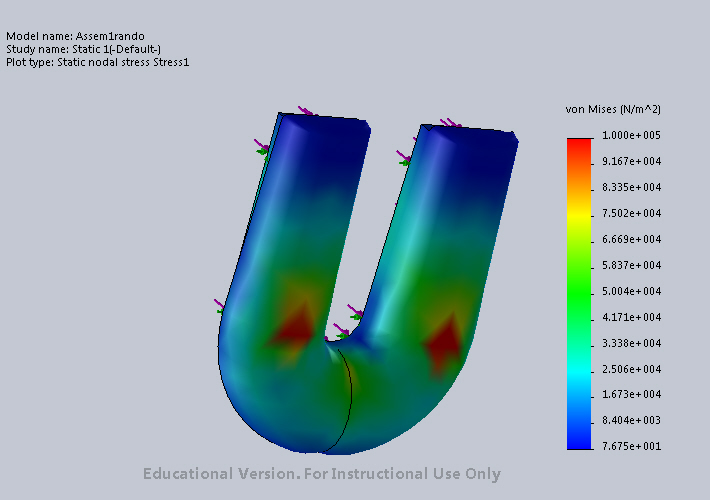
\includegraphics[width=2.5in]{pics/buttocksPressureMax.jpg}
    \caption{stress results for simulation with maximum peak stress}
    \label{maxstress}
\end{figure}

The results of the tests were documented and the raw numbers were extracted to allow for further data analysis. The important values of the peak stress on the bottom surface of the buttocks model were documented as were the average stresses over the bottom surface. These results can be seen in table \ref{resultsRaw}.

\begin{table}[!t]
    \centering
    \caption{Raw results}
    \label{resultsRaw}
    \begin{tabular}{llll}
    \hline
     Young's Modulus  & Poisson's Ratio & Avg stress & Max stress \\ \hline \hline
    10000000          & 0.49            & 25975        & 169400       \\ \hline 
    1000000           & 0.49            & 23791        & 79706        \\ \hline
    100000            & 0.49            & 14737        & 42120        \\ \hline
    10000             & 0.49            & 28175        & 23060        \\ \hline
    10000000          & 0.394           & 25885        & 142000       \\ \hline
    1000000           & 0.394           & 21936        & 66040        \\ \hline
    100000            & 0.394           & 13905        & 34600        \\ \hline
    10000             & 0.394           & 26271        & 21330        \\ \hline
    10000000          & 0.25            & 25881        & 141280       \\ \hline
    1000000           & 0.25            & 20337        & 61252        \\ \hline
    100000            & 0.25            & 12525        & 33740        \\ \hline
    10000             & 0.25            & 28428        & 21680        \\ \hline
    10000000          & 0.1             & 25847        & 144290       \\ \hline
    1000000           & 0.1             & 19600        & 60730        \\ \hline
    100000            & 0.1             & 12121        & 33410        \\ \hline
    10000             & 0.1             & 28273        & 23190        \\ \hline
    10000000          & 0.05            & 25831        & 145620       \\ \hline
    1000000           & 0.05            & 19578        & 61058        \\ \hline
    100000            & 0.05            & 12474        & 33400        \\ \hline
    10000             & 0.05            & 27858        & 24520        \\ \hline
    \end{tabular}
\end{table}

Some trends emerged from the tabled data and the results were graphed to provide a more visually appealing understanding of the data. Using the various Poisson's ratio values a graph of the comparative peak stresses could be created. See figure \ref{peakstressPR} for a detailed graph of the peak stresses as compared to the Poisson's ratios.

\begin{figure}[!t]
\centering
 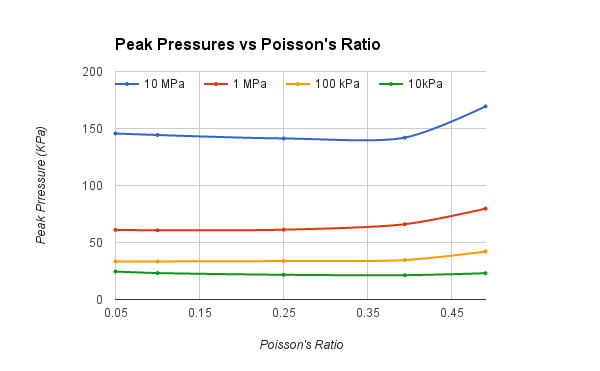
\includegraphics[width=2.5in]{pics/PeakPressurePR.png}
    \caption{Peak stresses for various Poisson's ratio values}
    \label{peakstressPR}
\end{figure}

Additionally graphs of the peak stresses as compared to the Young's modulus illustrated the relationship between these two properties. The x axis was kept at a log scale so as to better demonstrate the trend and also handle the large range of Young's modulus values. 

\begin{figure}[!t]
\centering
 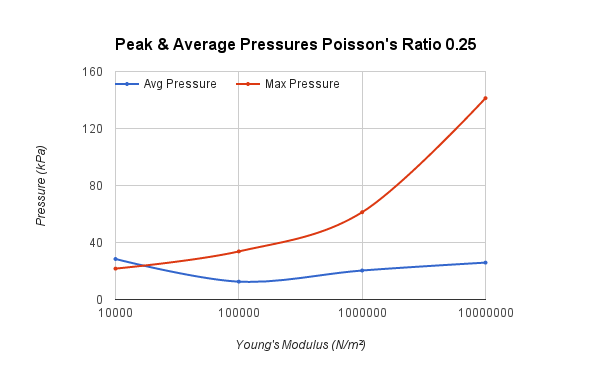
\includegraphics[width=2.5in]{pics/PeakPressureYM.png}
    \caption{Peak and average stresses for various Young's modulus values}
    \label{peakstressYM}
\end{figure}


\section{Discussion/Analysis}
% discuss results of flat cushion
The initial results from the flat cushion testing produced some interesting and important results for understanding the mechanisms behind the compression and stress propagation of the cushion material properties. As the material properties were changed some distinct trends emerged regarding the two main properties tested. Those were the Poisson's ratio and the Young's modulus. As the results show the Young's modulus had the greatest effect on the compression of the cushion and the stress levels on the underside of the buttocks model. The highest Young's modulus value of 10 MN/m\textsuperscript{2} produced the highest peak stress levels reaching 169 kN/m\textsuperscript{2} as can be seen in table \ref{resultsRaw}. The Piosson's ratio for this result just so happened to be set at 0.49. This upper limit for Young's modulus did not quite reach the possible maximums for polyurethane foam specifications (see table \ref{properties}) however it was high enough for the purpose of this simulation. These results also showed the peak stress occurring on two main points in the buttocks model in a comparable area to the ischial tuberosities and agree with stress profiles in previous studies \cite{HermanMiller2013,Nigel2002}. This indicates that the simulation is, at the least, producing a pressure profile that is similar to real world use. What wasn't comparable to similar studies is the magnitude of the maximum stress, which was much greater than any other study. This could be explained by the fact that these studies were attempting to decrease maximum stresses, rather than test the maximum stresses possible. This remains an unanswered question but something that does not necessarily undermine the whole study.

The material properties that resulted in the lowest peak stresses were when the Young's modulus was at it's lowest. With the Young's modulus set at 10 kN/m\textsuperscript{2} and the Poisson's ratio set at 0.394 the peak stress on the underside of the buttocks model reached only 21 kN/m\textsuperscript{2}. This can be seen in figure \ref{stress} and table \ref{resultsRaw}. This agrees with maximum stress levels of buttocks in previous studies \cite{Nigel2002}. This is more evidence to suggest that the simulation accurately mimics the real world in terms of maximum stresses observed when attempting to minimise them. Observing figure \ref{stress} the stress concentrations are a lot lower and more spread out. Therefore the trend is clear, keep the Young's modulus as low as possible however with the Poisson's ratio the trend is less clear. 

There are some broader points to discuss concerning the Poisson's ratio. Varying the ratio did not achieve a significant difference in stress distribution, or at least not anywhere near comparable to the variances achieved through varying the Young's modulus. The effect was small and it was difficult to determine a trend in any direction (see figure \ref{peakstressPR}). There did seem to be a shift upwards in peak stress as the Poisson's ratio became greater than 0.35 but at a lower Young's modulus value the effect was less pronounced. Another point which needs to be made is that although polyurethane foam has a range of Poisson's ratio between 0.3 and 0.7 (see table \ref{properties}) the Solidworks simulation only did a range from 0.05 to 0.49. This was partly due to the limitations of Solidworks, the software was unable to simulate any material with a Poisson's ratio of 0.5 or greater. Although initially thought of as a problem the results indicate that beyond 0.49 the peak stresses are far more likely to increase than decrease, therefore the lack of higher Poisson's ratio testing is not a complete loss. The initial recommendation for the ideal Poisson's ratio is not clear but it would seem a mid range of between 0.3 and 0.4 is desirable as that saw the lowest peak stress levels.


%discuss results of contoured cushion

    \subsection{Limitations}
    With the simulations being restricted to linear analysis we are in effect ignoring the non linearity characteristics of polyurethane foam. Foam has a compression profile of linearity up to a point but the the compression behaviour changes drastically. 
    
  %insert graph of foam stress profile
  
    The simulations never seemed to reach the point of compressing further than the bottom restraint so the assumption is that the model stayed within the range of linearity in compression of foam. However a more thorough analysis would test the same properties through a non linear simulation as this particular property may in fact be desirable for better comfort.

    Modelling the human body is a complex process. The body contains many variable solids, liquids and gases, each with their own material properties. On top of this the human body is not completely static and is constantly moving, circulating, breathing, whether voluntarily or not. The current simulations simplify the human buttocks down to a single solid, with uniform properties, with a single force pushing down uniformly. A more thorough investigation would begin to simulate the buttocks more completely s has been done in some studies \cite{Shu2009}. Alternatively commercially available human Solidworks models are may also be used to acquire more thorough results.
    %insert reference to Solidworks zygote
    
    %talk about limitations of poissons ratio in solidworks. mention the graphs indicate thats not too much of a problem
    

\section{Conclusion}
Knowing that a peak stress greater than 12kPa greatly increases discomfort in a sitting position Solidworks simulations were used to design a cushion that would reduce those peak stresses below this threshold. It was found that, of the material properties of the cushion, a lower Young's modulus allowed for lower peak stresses. 





% if have a single appendix:
%\appendix[Proof of the Zonklar Equations]
% or
%\appendix  % for no appendix heading
% do not use \section anymore after \appendix, only \section*
% is possibly needed

% use appendices with more than one appendix
% then use \section to start each appendix
% you must declare a \section before using any
% \subsection or using \label (\appendices by itself
% starts a section numbered zero.)
%


% \appendices
% \section{Proof of the First Zonklar Equation}


% use section* for acknowledgement
% \section*{Acknowledgment}


% The authors would like to thank...


% Can use something like this to put references on a page
% by themselves when using endfloat and the captionsoff option.
\ifCLASSOPTIONcaptionsoff
  \newpage
\fi



% trigger a \newpage just before the given reference
% number - used to balance the columns on the last page
% adjust value as needed - may need to be readjusted if
% the document is modified later
%\IEEEtriggeratref{8}
% The "triggered" command can be changed if desired:
%\IEEEtriggercmd{\enlargethispage{-5in}}

% references section

% can use a bibliography generated by BibTeX as a .bbl file
% BibTeX documentation can be easily obtained at:
% http://www.ctan.org/tex-archive/biblio/bibtex/contrib/doc/
% The IEEEtran BibTeX style support page is at:
% http://www.michaelshell.org/tex/ieeetran/bibtex/
\bibliographystyle{IEEEtran}
% argument is your BibTeX string definitions and bibliography database(s)
\bibliography{IEEEabrv,ref.bib}




% You can push biographies down or up by placing
% a \vfill before or after them. The appropriate
% use of \vfill depends on what kind of text is
% on the last page and whether or not the columns
% are being equalized.

%\vfill

% Can be used to pull up biographies so that the bottom of the last one
% is flush with the other column.
%\enlargethispage{-5in}




% that's all folks
\end{document}


